\documentclass[11pt,letterpaper,twoside,english]{article}

\usepackage[margin=1.4in]{geometry} % controls the size of the margins

% Special symbols, etc.
\usepackage{amssymb,amsbsy,latexsym,ytableau}
\usepackage{amsmath}
\usepackage{graphics, subfigure, float} 
\usepackage{cancel}
%\usepackage{todonotes}
% Encoding settings
\usepackage[latin1]{inputenc}
\usepackage[american]{babel}
\usepackage[T1]{fontenc} 
\usepackage{tikz}

\usepackage{titling} % allows posttitle command

% AMS Math packages

\usepackage{amscd,amsthm}

\usepackage{verbatim, comment} % can comment out text 
\usepackage{mdwlist} 

% Graphics
%\usepackage[dvips]{graphicx,epsfig,color}
%\usepackage{subfigure}
%\usepackage{pst-all}
%\usepackage{pstricks-add}
\usepackage{hyperref}  % can only be used with pdflatex - gives hyperlinks
\usepackage{bm} % bold math font
\usepackage{bbm}
\usepackage{pgfplots}

\usepackage{todonotes}

\newtheoremstyle{theorem}{1em}{1em}{\slshape}{0pt}{\bfseries}{.}{ }{}
\theoremstyle{theorem}
\newtheorem{theorem}{Theorem}[section]
\newtheorem*{theorem*}{Theorem}
\newtheorem{corollary}[theorem]{Corollary}
\newtheorem{proposition}[theorem]{Proposition}
\newtheorem{lemma}[theorem]{Lemma}
\newtheorem{claim}[theorem]{Claim}
\newtheorem{conjecture}[theorem]{Conjecture}
\newtheorem{definition}[theorem]{Definition}
\newtheorem*{claim*}{Claim}

\theoremstyle{remark}
\newtheorem{remark}[theorem]{Remark}
\newtheorem*{remark*}{Remark}
\newtheorem{algorithm}{Algorithm}
\newtheorem*{question*}{Question}
\newtheorem{question}{Question}
\newtheorem{example}[theorem]{Example}

\providecommand{\R}{\mathbb{R}}

\providecommand{\setN}{\mathbb{N}}
\providecommand{\setZ}{\mathbb{Z}}
\providecommand{\setQ}{\mathbb{Q}}
\providecommand{\setR}{\mathbb{R}}
\providecommand{\E}{\mathrm{E}}
\providecommand{\Pr}{\mathrm{Pr}}
\providecommand{\Var}{\mathrm{Var}}

\tikzset
{
    treenode/.style = {circle, draw=black, align=center, minimum size=1cm},
}

\makeatother

\title{Almost Orthogonal vectors} 

\author{Yajit Jain, Deepak Narayanan, Leon Zhang}

\begin{document}

\maketitle

\section{Introduction}
Given a dimension $n$ and a number $N > n$ of vectors, we want to find vectors $v_1, v_2, \ldots, v_N \in \mathbb{R}^n$ of unit length, such that
$$\epsilon = \max_{i \neq j} \{ |v_i \cdot v_j|^2 \}$$
is as small as possible.

\section{$n=2$, generic $N$}
In this section, we consider the problem of almost orthogonal vectors of dimensionality $2$.

It is obvious that for $N=2$, we can find an $\epsilon$ equal to $0$, since it easy to pick two unit vectors $v_1$ and $v_2$ of unit length that are orthogonal to each other -- a simple example of such vectors is $[1, 0]^T$ and $[0, 1]^T$. 

However, we see that the problem gets harder for larger $N$. Let us first consider the specific case of $N=3$; once we build some intuition for the problem, we will try to generalize to generic $N$.
\\

It's clear that when $N=3$, the value of $\epsilon$ must be greater than $0$, since there is no way three dimensionality-$2$ vectors can be orthogonal to each other.

In addition, we see that for $N=3$, the quantity $\epsilon$ for three unit-length vectors $v_1, v_2, v_3 \in \mathbb{R}^2$ is given by $$\max \{ |v_1 \cdot v_2|^2, |v_1 \cdot v_3|^2, |v_2 \cdot v_3|^2 \}$$

Since we don't care about the sign of the dot product between any two vectors, if we define the unit vectors $v_4, v_5, v_6 \in \mathbb{R}^2$ to be the reverses of $v_1, v_2, v_3$ respectively, then we see that $\epsilon$ can be equivalently expressed as $$\max_{i \neq j} \{|v_i \cdot v_j |^2 \}$$
where $i, j \in \{1,2,\ldots,6\}$ -- the above result holds because if the vector $\mathcal{R}(v)$ is the reverse of the vector $v$, then $|v \cdot v'| = |\mathcal{R}(v) \cdot v'|$ for some arbitrary vector $v'$.

Without loss of generality, let $x_1 = [1, 0]^T$; then since $x_4$ is the reverse of $x_1$, we see that $x_4 = [-1, 0]^T$. Also, without loss of generality assume that $x_2$ and $x_3$ are above the $x$-axis, and that $x_2$ is to the right of $x_3$.

\begin{figure}[!h]
    \centering
    \begin{tikzpicture}[yscale=-1] 
        % x-axis
        \draw [thick,->] (-4.5, 0) -- (4.5, 0);
        % y-axis
        \draw [thick,->] (0, 4.5) -- (0, -4.5);
        % origin label
        \node at (-0.5, 0.3) {\text{$(0, 0)$}};
        % x-axis label
        \node at (4.5, 0.5) {\text{$x$}};
        % y-axis label
        \node at (0, -5) {\text{$y$}};
        % circle
        \draw (0,0) circle (3cm);
        \draw (3,0)[blue,fill=blue] circle (0.1cm);
        \draw (1.5, -2.59)[blue,fill=blue] circle (0.1cm);
        \draw (-1.5, -2.59)[blue,fill=blue] circle (0.1cm);
        
        \draw [thick,-,blue] (3, 0) -- (0, 0);
        \draw [thick,-,blue] (1.5, -2.59) -- (0, 0);
        \draw [thick,-,blue] (-1.5, -2.59) -- (0, 0);
        
        \node at (4, -0.3) {\text{$x_1 = [1,0]$}};
        \node at (2.8, -3.1) {\text{$x_2 = [\cos \pi/3,\sin \pi/3]$}};
        \node at (-2.8, -3.1) {\text{$x_3 = [\cos 2\pi/3,\sin 2\pi/3]$}};
    \end{tikzpicture}
    \caption{A configuration of three unit vectors that produce the optimum $\epsilon$ for $n=2, N=3$}
\end{figure}


Let $\theta_1$ be the angle between $x_1$ and $x_2$, $\theta_2$ be the angle between $x_2$ and $x_3$ and $\theta_3$ be the angle between $x_3$ and $x_4$. Now, it is easy to see that $\theta_1 + \theta_2 + \theta_3 = \pi$ and that $$\epsilon = \max_{i \in \{1,2,3\}} \cos ^2 \theta_i$$

Before proceeding, we state and prove the following lemma.
\begin{lemma}
Consider $n$ angles $\theta_1, \theta_2, \ldots, \theta_n \in [0, \pi]$ s.t. $\theta_1 + \theta_2 + \ldots + \theta_n = \pi$. Then $\epsilon = \max_i \cos^2 \theta_i$ must equal $\cos^2 \theta_j$ where $j = \text{argmin }\theta_i$.
\end{lemma}

\begin{proof}

\begin{figure}[!h]
	\centering
	\begin{tikzpicture}
		\begin{axis}[%
			axis x line=center, axis y line=center,
			width=10cm,
			height=4cm,
			scale only axis,
			xmin=-5,
			xmax=5,
			xtick={1.57,  3.14, 4.71},
			xticklabels={, $\pi$, },
			extra x ticks={-4.71, -3.14, -1.57},
			extra x tick labels={, $-\pi$,},
			extra x tick style={
			    xticklabel style={yshift=0.5ex, anchor=south}
			},
			ymin=-1.4,
			ymax=1.4,
			ytick={-1,  0,  1}]]
			\addplot[domain=-2*pi:2*pi,smooth] (\x,{cos(\x r)});
		\end{axis}
	\end{tikzpicture}
	\caption{Plot of $\cos \theta$ versus $\theta$}
\end{figure}

Our arguments will hinge on the fact that for all $\theta \in [0, \pi/2]$, the function $\cos \theta$ is decreasing -- this is easy to see from Figure $2$. Without loss of generality, let us assume that $\theta_1 \geq \theta_2 \geq \ldots \geq\theta_n$. Hence we want to prove that $\epsilon$ is equal to $\cos^2 \theta_n$.

We split our proof into two cases,
\begin{itemize}
\item $\theta_1, \theta_2, \ldots, \theta_n \in [0, \pi/2]$: In this case, it is easy to see that $\epsilon = \cos^2 \theta_n$ from the fact that $\cos \theta$ is a decreasing function in $\theta$ if $\theta \in [0, \pi/2]$.

\item One of $\theta_1, \theta_2, \dots, \theta_n$ is greater than $\pi/2$:

Then, if $\theta_1 > \pi/2$ we see that $\cos^2 \theta_1 = \cos^2 (\pi - \theta_1)$ is equal to $\cos^2 (\theta_2 + \theta_3 + \ldots + \theta_n)$. Furthermore, $\pi - \theta_1 = \theta_2 + \theta_3 + \ldots + \theta_n < \pi/2$, which means $\cos^2 \theta_1 = \cos^2 (\theta_2 + \theta_3 + \ldots + \theta_n) < \cos^2 \theta_n$. (since $\theta_n < \theta_2 + \theta_3 + \ldots + \theta_n$)

In addition, we see that for all $i \in \{2, 3, \ldots, n-1\}$, $\cos^2 \theta_i < \cos^2 \theta_n$, from which we can conclude that in this case too, $\epsilon$ is equal to $\cos^2 \theta_n$.

\end{itemize}
\end{proof}

From the above lemma, we can conclude that if $j = \text{argmin } \theta_i$ and $\theta_1 + \theta_2 + \theta_3 = \pi$, then $\epsilon = \cos^2 \theta_j$.

Furthermore, we can obtain an upper bound on $\theta_j$ by observing that $\theta_ 1 + \theta_ 2 + \theta_3 \geq \theta_ j + \theta_j + \theta_j = 3 \theta_j \Rightarrow \theta_j \leq \pi/3$. Since we're interested in the smallest such $\epsilon$ and since the cosine function is a decreasing function in $\theta$ between $0$ and $\pi/2$, we conclude that the optimum value of $\epsilon$ for $n=2$ and $N=3$ is $\cos^2 \pi / 3$. Figure $1$ shows this optimum configuration.

\begin{theorem}
For $n=2$ and arbitrary $N$, the optimum value of $\epsilon$ is given by $\cos^2 \pi/N$.
\end{theorem}

\begin{proof}
The proof of this theorem is similar to the proof for the specific case of $N=3$.

Again without loss of generality, we can assume that the vectors $x_1, x_2, \ldots, x_N$ are on or above the $x$-axis, and that $x_1 = [1,0]^T$ and that $x_{N+1} = [-1,0]^T$ -- if any vector $x_i$ were not above the $x$-axis, then we could just consider its reverse.

Let us define $\theta_i$ as the angle between the vectors $x_i$ and $x_{i+1}$. Then, we quickly see that $\theta_1 + \theta_2 + \ldots + \theta_N = \pi$. If $j = \text{argmin } \theta_i$, $\epsilon = \cos^2 \theta_j$.

Since $\theta_ 1 + \theta_2 + \ldots + \theta_N \geq N \cdot \theta_j \Rightarrow \theta_j \leq \pi/N$, we conclude that the optimum $\epsilon$ value is in fact equal to $\cos^2 \pi/N$.
\end{proof}

\begin{figure}[!h]
    \centering
    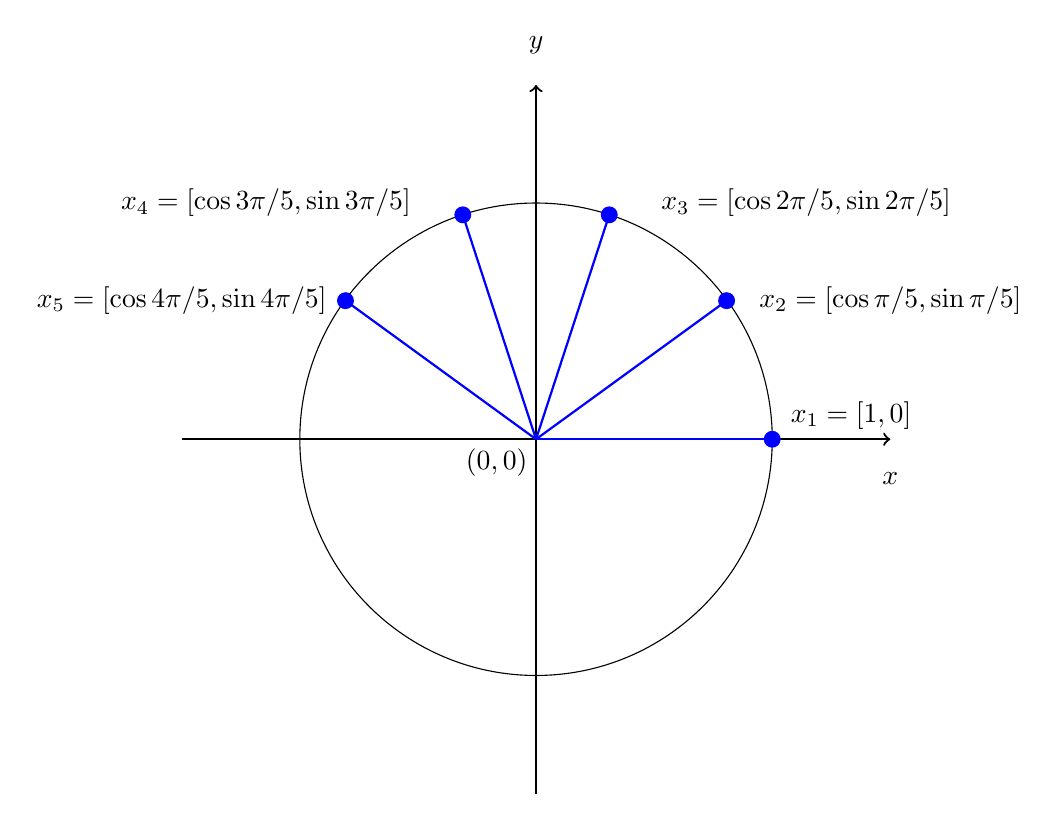
\begin{tikzpicture}[yscale=-1] 
        % x-axis
        \draw [thick,->] (-4.5, 0) -- (4.5, 0);
        % y-axis
        \draw [thick,->] (0, 4.5) -- (0, -4.5);
        % origin label
        \node at (-0.5, 0.3) {\text{$(0, 0)$}};
        % x-axis label
        \node at (4.5, 0.5) {\text{$x$}};
        % y-axis label
        \node at (0, -5) {\text{$y$}};
        % circle
        \draw (0,0) circle (3cm);
        \draw (3,0)[blue,fill=blue] circle (0.1cm);
        \draw (2.42, -1.76)[blue,fill=blue] circle (0.1cm);
        \draw (0.93, -2.85)[blue,fill=blue] circle (0.1cm);
        \draw (-2.42, -1.76)[blue,fill=blue] circle (0.1cm);
        \draw (-0.93, -2.85)[blue,fill=blue] circle (0.1cm);
        
        \draw [thick,-,blue] (3, 0) -- (0, 0);
        \draw [thick,-,blue] (2.42, -1.76) -- (0, 0);
        \draw [thick,-,blue] (0.93, -2.85) -- (0, 0);
        \draw [thick,-,blue] (-2.42, -1.76) -- (0, 0);
        \draw [thick,-,blue] (-0.93, -2.85) -- (0, 0);
        
        \node at (4, -0.3) {\text{$x_1 = [1,0]$}};
        \node at (4.5, -1.76) {\text{$x_2 = [\cos \pi/5,\sin \pi/5]$}};
        \node at (3.43, -3) {\text{$x_3 = [\cos 2\pi/5,\sin 2\pi/5]$}};
         \node at (-4.5, -1.76) {\text{$x_5 = [\cos 4\pi/5,\sin 4\pi/5]$}};
        \node at (-3.43, -3) {\text{$x_4 = [\cos 3\pi/5,\sin 3\pi/5]$}};
    \end{tikzpicture}
    \caption{A configuration of five unit vectors that produce the optimum $\epsilon$ for $n=2, N=5$}
\end{figure}

\begin{figure}[!h]
    \centering
    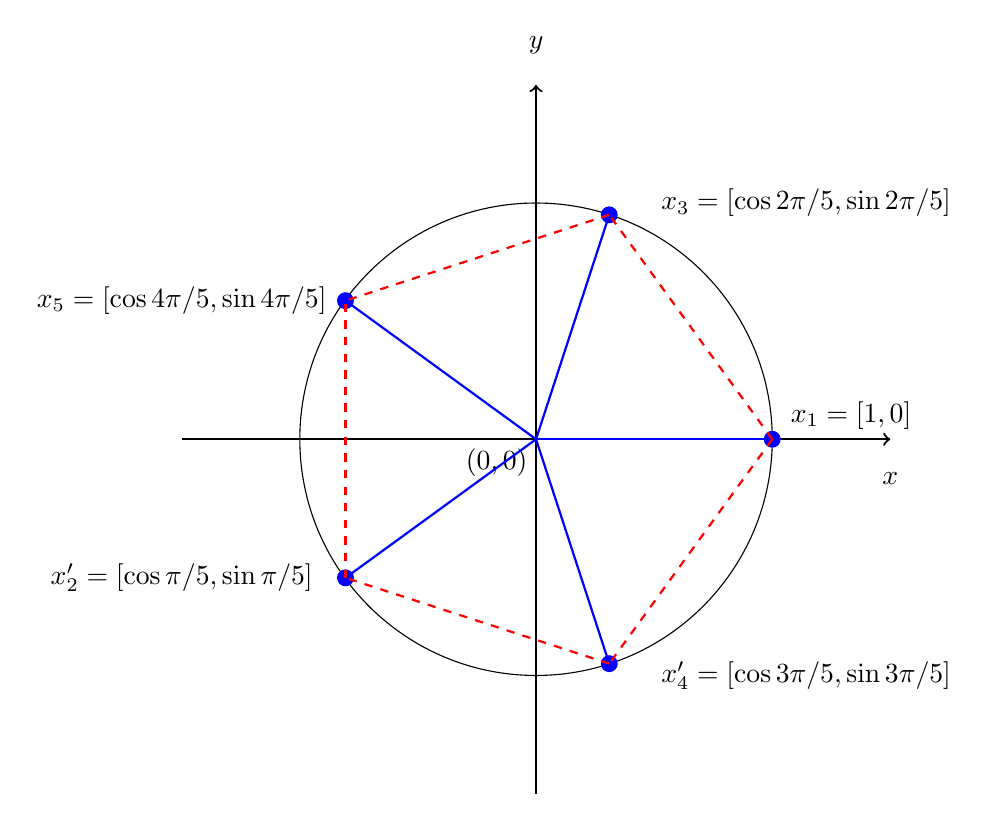
\begin{tikzpicture}[yscale=-1] 
        % x-axis
        \draw [thick,->] (-4.5, 0) -- (4.5, 0);
        % y-axis
        \draw [thick,->] (0, 4.5) -- (0, -4.5);
        % origin label
        \node at (-0.5, 0.3) {\text{$(0, 0)$}};
        % x-axis label
        \node at (4.5, 0.5) {\text{$x$}};
        % y-axis label
        \node at (0, -5) {\text{$y$}};
        % circle
        \draw (0,0) circle (3cm);
        \draw (3,0)[blue,fill=blue] circle (0.1cm);
        \draw (-2.42, 1.76)[blue,fill=blue] circle (0.1cm);
        \draw (0.93, -2.85)[blue,fill=blue] circle (0.1cm);
        \draw (-2.42, -1.76)[blue,fill=blue] circle (0.1cm);
        \draw (0.93, 2.85)[blue,fill=blue] circle (0.1cm);
        
        \draw [thick,-,blue] (3, 0) -- (0, 0);
        \draw [thick,-,blue] (-2.42, 1.76) -- (0, 0);
        \draw [thick,-,blue] (0.93, -2.85) -- (0, 0);
        \draw [thick,-,blue] (-2.42, -1.76) -- (0, 0);
        \draw [thick,-,blue] (0.93, 2.85) -- (0, 0);
        
        \node at (4, -0.3) {\text{$x_1 = [1,0]$}};
        \node at (-4.5, 1.76) {\text{$x'_2 = [\cos \pi/5,\sin \pi/5]$}};
        \node at (3.43, -3) {\text{$x_3 = [\cos 2\pi/5,\sin 2\pi/5]$}};
         \node at (-4.5, -1.76) {\text{$x_5 = [\cos 4\pi/5,\sin 4\pi/5]$}};
        \node at (3.43, 3) {\text{$x'_4 = [\cos 3\pi/5,\sin 3\pi/5]$}};
        
        \draw [thick,-,red,dashed] (3, 0) -- (0.93, 2.85);
        \draw [thick,-,red,dashed] (3, 0) -- (0.93, -2.85);
        \draw [thick,-,red,dashed] (0.93, 2.85) -- (-2.42, 1.76);
        \draw [thick,-,red,dashed] (0.93, -2.85) -- (-2.42, -1.76);
        \draw [thick,-,red,dashed] (-2.42, 1.76) -- (-2.42, -1.76);
    \end{tikzpicture}
    \caption{A configuration of five unit vectors that produce the optimum $\epsilon$ for $n=2, N=5$ with $x_2$ and $x_4$ from the previous figure reversed}
\end{figure}

Figure $3$ shows an optimum configuration for $n=2$ and $N=5$. Note by taking reflections of $x_2$ and $x_4$ instead, we get five vectors that form a regular $5$-gon -- this can be seen in Figure $4$. This can be done for all odd $N$; unfortunately, even $N$ do not produce such nice polygons.

\section{The Parallelogram Law}

First we give the definition of the norm on vectors in $\R^n$ in terms of the dot product:

\begin{definition}
For a vector $v\in\R^n$ the norm of $v$ is the positive value of $||v||$ given by the equation
$$
||v||^2=v\cdot v.
$$
\end{definition}
\begin{theorem}[Parallelogram Law]
For vectors $v_1,\cdots,v_n\in\R^n$, the following identity holds
$$
||v_1+\cdots+v_n||^2=\displaystyle\sum_{i=1}^n||v_i||^2+2\displaystyle\sum_{1\le i<j\le n}v_i\cdot v_j.
$$
\proof
First consider the following identity from the definition of the norm for vectors $u,v\in\R^n$:
$$
||u+v||^2=(u+v)\cdot (u+v)=u\cdot u+u\cdot v+ v\cdot u + v\cdot v=||u||^2+||v||^2+2u\cdot v.
$$
Now if we let $u=v_1$ and $v= v_2+\cdots+v_n$ we get 
$$
||v_1+v_2+\cdots+v_n||^2=||v_1||^2+||v_2+\cdots +v_n||^2+2\sum_{i=2}^n v_1\cdot v_i.
$$
If we recurse on $||v_2+\cdots +v_n||^2$ using induction we get the desired result. 
\end{theorem}


\section{$(n,n+1)$}
Let us consider the situation in which we try to minimize $\epsilon$ for $n+1$ vectors in an $n$ dimensional space. First we introduce the definition of a simplex, and then we will proceed to characterize $\epsilon$ in this case. 

\begin{definition}
An $n$-dimensional simplex is given by the convex hull of the $n+1$ points in $\R^{n+1}$ described as having a 1 in a single coordinate and zeros in every other coordinate. 
\end{definition}

Here are diagrams of a 2-dimensional simplex:

\begin{figure}[!h]
    \centering
        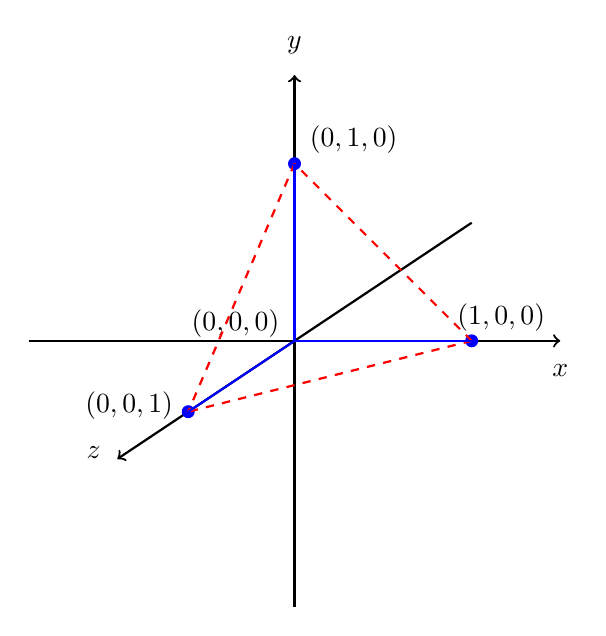
\begin{tikzpicture}[yscale=-1, scale=0.75]
        % x-axis
        \draw [thick,->] (-4.5, 0) -- (4.5, 0);
        % y-axis
        \draw [thick,->] (0, 4.5) -- (0, -4.5);
        % z-axis
        \draw [thick, ->] (3.0, -2.0) -- (-3.0, 2.0);
        % origin label
        \node at (-1, -0.3) {\text{$(0, 0, 0)$}};
        % x-axis label
        \node at (4.5, 0.5) {\text{$x$}};
        % y-axis label
        \node at (0, -5) {\text{$y$}};
         % z-axis label
        \node at (-3.4, 1.9) {\text{$z$}};
        \node at (3.5, -0.4) {\text{$(1, 0, 0)$}};
        \node at (1, -3.4) {\text{$(0, 1, 0)$}};
        \node at (-2.8, 1.1) {\text{$(0, 0, 1)$}};
        % circle
        \draw (3,0)[blue,fill=blue] circle (0.1cm);
        \draw (0, -3)[blue,fill=blue] circle (0.1cm);
        \draw (-1.8, 1.2)[blue,fill=blue] circle (0.1cm);
        
        \draw [thick,-,red,dashed] (3, 0) -- (0, -3);
        \draw [thick,-,red,dashed] (0, -3) -- (-1.8, 1.2);
        \draw [thick,-,red,dashed] (3, 0) -- (-1.8, 1.2);
        
        \draw [thick,-,blue] (3, 0) -- (0, 0);
        \draw [thick,-,blue] (0, -3) -- (0, 0);
        \draw [thick,-,blue] (-1.8, 1.2) -- (0, 0);
    \end{tikzpicture}
    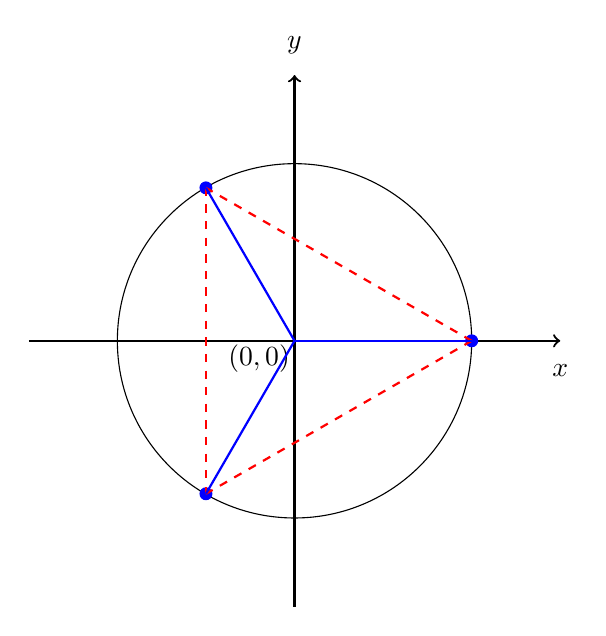
\begin{tikzpicture}[yscale=-1, scale=0.75]
        % x-axis
        \draw [thick,->] (-4.5, 0) -- (4.5, 0);
        % y-axis
        \draw [thick,->] (0, 4.5) -- (0, -4.5);
        % origin label
        \node at (-0.6, 0.3) {\text{$(0, 0)$}};
        % x-axis label
        \node at (4.5, 0.5) {\text{$x$}};
        % y-axis label
        \node at (0, -5) {\text{$y$}};
        % circle
        \draw (0,0) circle (3cm);
        \draw (3,0)[blue,fill=blue] circle (0.1cm);
        \draw (-1.5, 2.59)[blue,fill=blue] circle (0.1cm);
        \draw (-1.5, -2.59)[blue,fill=blue] circle (0.1cm);
        
        \draw [thick,-,red,dashed] (3, 0) -- (-1.5, 2.59);
        \draw [thick,-,red,dashed] (3, 0) -- (-1.5, -2.59);
        \draw [thick,-,red,dashed] (-1.5, -2.59) -- (-1.5, 2.59);
        
        \draw [thick,-,blue] (3, 0) -- (0, 0);
        \draw [thick,-,blue] (-1.5, 2.59) -- (0, 0);
        \draw [thick,-,blue] (-1.5, -2.59) -- (0, 0);
    \end{tikzpicture}

    \caption{A 2-dimensional simplex drawn in $\R^3$ on the left, and then centered at the origin in $\R^2$ on the right.}
\end{figure}

Before proceeding with the theorem, we notice that when $n=2$, the configuration of $N=3$ vectors that produced the minimum value of $\epsilon$ made up a simplex centered at the origin. 


\begin{theorem}
If $N=n+1$ and the vectors in question are denoted $v_1,\cdots, v_N$, then over all configurations of these vectors the maximum value of $v_i\cdot v_j$ for $i\neq j$ is $\frac{-1}{n}$. This is achieved when the vectors are arranged in an $n$ dimensional simplex centered at the origin, and in this configuration $\epsilon=\frac{1}{n^2}$.  
\end{theorem}

\proof
Let $\delta=\max_{i\neq j}\{v_i\cdot v_j\}$. We first show that $\delta\le-\frac{1}{n}$ by showing that the origin-centered simplex configuration of the vectors $v_1,\cdots v_N$ produces a value $\delta=-\frac{1}{n}$. 

We must first describe the vectors that make up the origin centered simplex. To center our simplex at the origin we take each vector in the original simplex, and subtract from it the centroid of the original simplex. The centroid of the original simplex takes the form $(\frac{1}{n},\frac{1}{n},\cdots,\frac{1}{N})$, so the points of the new simplex take the form
$$
\left(-\frac{1}{N},\cdots,-\frac{1}{N},\frac{N-1}{N},-\frac{1}{N},\cdots,-\frac{1}{N}\right).
$$
If we renormalize these vectors we get 
$$
\sqrt{\frac{N}{N-1}}\left(-\frac{1}{N},\cdots,-\frac{1}{N},\frac{N-1}{N},-\frac{1}{N},\cdots,-\frac{1}{N}\right).
$$
If we take the dot product of any two such vectors we get
$$
\frac{N}{N-1}\left(-2\cdot\frac{N-1}{N^2}+(N-2)\cdot\frac{1}{N^2}\right)=\frac{N}{N-1}\cdot-\frac{1}{N}=-\frac{1}{N-1}=-\frac{1}{n}.
$$
So an upper bound on the value of $\delta$ for all configurations of $n+1$ vectors in $n+1$ dimensional space is $\delta\le\frac{-1}{n}$. 

To see that $\delta\ge-\frac{1}{n}$ we use the parallelogram law. Recall that the parallelogram law states that 

$$
||v_1+\cdots+v_{n+1}||^2=\displaystyle\sum_{i=1}^{n+1}||v_i||^2+2\displaystyle\sum_{1\le i<j\le n+1}v_i\cdot v_j.
$$
In our case we know three things. First, since the vectors are arranged in a simplex, $v_1+\cdots+v_{n+1}=0$. Second, $v_i\cdot v_j\le\delta$ for any $i<j$. Third, $||v_i||=1$. Therefore 
$$
0\le n+1+n(n+1)\delta.
$$
This implies that $\delta\ge -\frac{1}{n}$ as desired. Now we see that $\delta=-\frac{1}{n}$, so $|\delta|=\frac{1}{n}$, and therefore $\epsilon=\frac{1}{n^2}$. 

\section{N>n+1}

We conjecture that in cases where $N>n+1$ we can never have an arrangement of the vectors where all values of $|v_i\cdot v_j|^2$ are the same. 

\section{Applications to sphere packing}
We should be able to prove something about the radius of spheres you can pack in the case of $N=n+1$, taking as intuition square and hexagonal tilings of the plane and cubic and tetrahedral tilings of 3-space. 

\end{document}